% !TEX encoding = UTF-8
% !TEX TS-program = pdflatex
% !TEX root = ../tesi.tex
% !TEX spellcheck = it-IT

%************************************************



Il \emph{Micro-blogging} è un nuovo mezzo di comunicazione che permette agli utenti di pubblicare in broadcast  costantemente e in  "real time" brevi contenuti digitali, come testo, link, immagini o video. 
Questi contenuti vengono pubblicati in una rete sociale, in cui ogni utente può generare nuove informazioni, aggiornare informazioni esistenti e condividere o commentare informazioni pubblicate da altri utenti \cite{Java:2007:WWT:1348549.1348556}.  

Negli ultimi anni, questo mezzo di comunicazione ha attirato l'attenzione di una vasta  comunità  di ricercatori e aziende che operano in diversi ambiti.
La popolarità crescente di questi servizi di micro-blogging è dovuta alla loro portabilità, immediatezza e facilità d'uso. Queste caratteristiche consentono agli utenti di interagire istantaneamente e diffondere informazioni.

Virtualmente qualsiasi persona che assiste o è coinvolta in un qualsiasi evento è capace, grazie a questi micro-blog, di diffondere informazioni durante l'accaduto stesso. Ad esempio, durante i recenti conflitti, crisi sociali e manifestazioni\footnote{e.g.: primavera araba, proteste iraniane del 2009, elezioni presidenziali, etc.}, milioni di persone hanno utilizzato sistemi di micro-blogging come Twitter sia per diffondere notizie che per ricevere aggiornamenti sugli ultimi accadimenti.

Twitter è ad oggi il servizio di micro-blogging più utilizzato in assoluto. Con circa 284 milioni di utenti attivi al mese, ogni giorno vengono prodotti oltre 500 milioni di tweets al giorno. Gli utenti di Twitter, possono inviare in broadcast brevi status (\emph{tweets}), non  più lunghi di 140 caratteri,
 ad una rete di utenti (\emph{follower}) attraverso diversi dispositivi (e.g. smartphones, web-app, email, etc.).
 
Se da un lato la dimensionalità dei tweet rappresenta per alcuni utenti un forte limite, dall'altro rappresenta una delle caratteristiche fondamentali di Twitter: \emph{l'immediatezza}. Questo vincolo costringe gli utenti a produrre messaggi molto sintetici, quasi come slogan, che quindi sono più facili da diffondere.

%Inoltre, sebbene  i tweet siano caratterizzati da un contenuto molto ristretto, bisogna considerare che milioni di persone  \emph{twittano}\footnote{http://www.garzantilinguistica.it/ricerca/?q=twittare}  da ogni parte del mondo, a proposito di argomenti più disparati da manifestazioni sportive a crisi globali.
Monitorare e analizzare questo flusso di  contenuti generati degli utenti può portare a scoprire informazioni molto utili. Per esempio, molte aziende utilizzano Twitter sia per pubblicizzare e raccomandare i loro prodotti, che comprendere  le opinioni dei loro clienti riguardo i loro prodotti (o dei loro competitor) .
Inoltre i tweet sono stati analizzati per predire i risultati delle votazioni presidenziali, crimini \cite{Wang2012}, attività terroristiche o eventi. In generale, un evento può essere definito \emph{qualcosa che accade in un luogo e tempo specifico}. 

Diversi lavori in letteratura si sono focalizzati sul problema di estrazione automatica di eventi, dimostrando l'importanza di Twitter come mezzo di comunicazione. Infatti in diverse occasioni si è osservato come le notizie relative ad eventi si diffondano prima e più velocemente delle notizie diffuse sui media tradizionali (come la morte di Micheal Jackson \footnote{ttp://www.dailymail.co.uk/sciencetech/article-1195651/How-Michael-Jacksons-death-shut- Twitter-overwhelmed-Google–killed-Jeff-Goldblum.html}).

Scoprire eventi da Twitter non è un task banale. Infatti, tweet associati ad  eventi, rappresentano solo una piccola percentuale di tutti i tweet prodotti. La maggior parte infatti, è costituita da status personali, messaggi anche privi di senso, opinioni, spam, etc..   
La maggior parte degli approcci esistenti per l'estrazione automatica di eventi, utilizza la similarità sintattica dei contenuti testuali dei tweets. Queste soluzioni non considerano né il problema della dimensionalità (mole di dati da processare) né tanto meno sfruttano informazioni contestuali quali tempo, luogo o entità coinvolte (e.g. persone o organizzazioni).

La mole dei dati da analizzare e la necessità di estrarre efficientemente risultati rendono il problema dell'estrazione di eventi assimilabile ad un problema  come  "Big Data Analytics".  
Obiettivo di questa tesi, è quello di proporre un sistema scalabile per il task di event detection a partire da twitter, utilizzando un'architettura di calcolo distribuita. Nella soluzione proposta oltre alla classica rappresentazione sintattica dei tweet, sarà adottata una rappresentazione semantica utilizzando la base di conoscenza di DBpedia.


\section{Twitter}
Molte notizie sono state diffuse su Twitter anche prima della diffusione sui media classici. Uno degli esempi più significati è stato rappresentato dalla notizia della di Michael Jackson del 2009. Alle 2:26pm
del 24 Giungo 2009, la notizia trapelò su Twitter e fu diffusa in una maniera così virale che che Google la identificò come un attacco hacker. La validità della notizia fù verificata da Google solo 25 minuti dopo,   solo allora i media mainstream iniziarono a far diffondere la notizia \footnote{ttp://www.dailymail.co.uk/sciencetech/article-1195651/How-Michael-Jacksons-death-shut-
Twitter-overwhelmed-Google–killed-Jeff-Goldblum.html}.Anche nel caso del terremoto in Abruzzo del 6 aprile 2009, gli utenti Twitter hanno segnalato la notizia prima dei media tradizionali. 
\section{Big Data}
Sebbene oggigiorno il termine \lq\lq big data\rq\rq sia molto in voga, la sua definizione è ancora piuttosto vaga. Alcuni definizioni fanno riferimento al volume dei dati, altre  invece fanno riferimento alla ricchezza dei dati. Per altri, i \lq\lq big data\rq\rq sono   quei dati troppo grandi per gli standard tradizionali, ovvero quando il volume dei dati supera petabytes o zettabytes. Altri ancora intendono per big data, quei dati che riescono ad esprimere più sfaccettature delle stesse entità che rappresentano, che se fossero memorizzati nei classici database relazionali (RDBMS) avrebbero migliaia di colonne. 
L'aggettivo \lq\lq big\lq\lq non si riferisce soltanto al volume dei dati, ma anche alla loro complessità. Esistono infatti, molti piccoli datasets che  sono considerati big data che non richiedono molo spazio di memorizzazione, ma hanno una complessità intrinseca molto alta. Allo stesso tempo, datasets che richiedono molto spazio di memorizzazione possono non essere abbastanza complessi, da essere considerati Big data. Il solo volume dei dati, quindi non basta a definire questi big-data. Una definizione molto diffusa è quella delle tre \emph{V}, dove, oltre al volume dei dati, si considera anche la Velocità e la Varietà .
Per Velocità si intende che i dati sono generati con un'elevata frequenza.
La Varietà si riferisce al fatto che i dati possono essere  strutturati, semi strutturati o non strutturati affatto : dati transazionali, video, audio testo file di log.
In aggiunta a queste tre V, talvolta viene aggiunta una quarta alla definizione: \emph{Veridicità}.
La veridicità è un indicazione dell'integrità di questi dati e si riferisce al livello di trust in questi dati stessi, affinché si possano utilizzare nei processi decisionali
Analizzare questi big-data può permettere  di prendere decisioni in maniera più oculata e molto più velocemente, usando dati che in passato erano inaccessibili o inutilizzabili.
Per tali ragioni, i classici database relazionali non riescono a gestire facilmente questi dati.
\subsection{Hadoop}
Hadoop è stato uno dei primi sistemi open-source più popolari per processare i big data.
\'E un sistema scalabile e fault-tolerant che consente di processare grandi dataset attraverso un cluster di server.  


\begin{figure}[h]
\centering
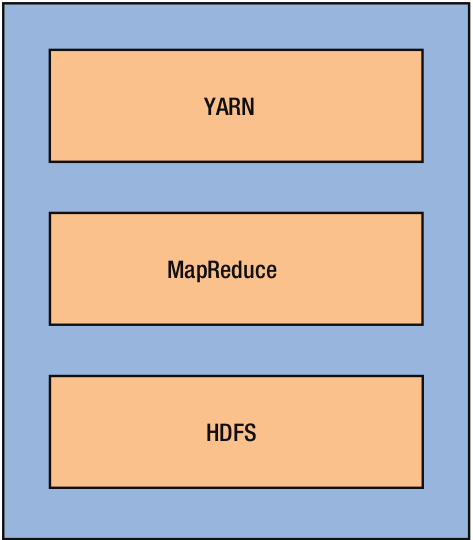
\includegraphics[width=0.4\textwidth]{hadoopCompo.png}
\caption{componenti principali di Hadooop}
\label{fig:hadoopComponets}
\end{figure} 
 
Uno dei fattori di successo di Hadoop è il basso costo. Hadoop è un sistema open-source che può essere eseguito su un cluster di commodity\footnote{hardware non dedicato di basso costo} hardware. Riesce cioè a garantire facilmente una scalabilità orizzontale aggiungendo al cluster, dei server poco costosi. Inoltre, riesce a garantire, via software la tolleranza ai guasti: assume che prima o poi vi saranno dei guasti e li gestisce in maniera trasparente. Uno sviluppatore software non dovrà preoccuparsi di gestire questi fault. Consente, cioè, di sviluppare applicazioni distribuite in maniera molto più semplice poiché viene sperata la logica di elaborazione dei dati dalla logica di distribuzione dei dati.
Hadoop è composto da tre componenti principali: un cluster mananger (YARN), un modello di computazione distribuito (Map-reduce) e un file system distribuito (HDFS)



 
 \subsubsection{Map Reduce}
 MapReduce è il modello di computazione distribuita fornito da Hadoop. Mentre HDFS fornisce un file system distribuito per memorizzare grandi dataset, MapReduce fornisce un framework di computazione che consente di processare grandi dataset in parallelo attraverso un cluster di computer (nodi). Questo modello astrae la computazione distribuita fornendo dei costrutti ad alto livello che consentono di sviluppare facilmente applicazioni distribuite.
 Il framework MapReduce schedula in maniera automatica l'esecuzione di un applicazione su un insieme di macchine in un cluster, prendendosi carico  della gestione della comunicazione fra nodi, del bilanciamento del carico di esecuzione fra i nodi e dei possibili guasti dei nodi.
In questo modo, gli sviluppatori possono concentrarsi sulla logica di processing dei dati tralasciando questi dettagli.

Come suggerisce il nome stesso, questo modello si basa su due funzioni :\emph{map}   e \emph{reduce}. Tutti i carichi di lavoro in un appplicazione MapReduce sono espressi implementando queste due funzioni.
La funzione \emph{map} riceve in input una coppia chiave-valore e restituisce a sua volta una insieme di  coppie chiave valore intermedie. Il framework MapReduce esegue la funzione map per ogni coppia chiave valore presente nel dataset di input. L'output delle funzioni Map, è ordinato e raggruppato in base ai valori di chiave intermedi, e costituirà l'input della funzione Reduce. La funzione \emph{Reduce} aggrega i risultati della funzione map, in base al valore di chiave intermedio.

I dati possono essere sia semi strutturati o non strutturati affatto, non è richiesto che i dati siano conformi ad uno schema rigido predefinito. L'unico requisito è che sia possibile esprimere il dataset in input come una serie di coppie chiave valore.
Il modello MapReduce ha rivoluzionato il modo di processare grandi datasets, offrendo un modello semplice che consente di scrivere programmi che possono essere eseguiti in parallelo su molte macchine. Grazie a questo, Map-Reduce consente di ottenere una scalabilità orizzontale: all'aumentare della dimensione dei dati è possibile aggiungere nuove macchine mantenendo quasi invariato il tempo di esecuzione.
\subsection{Apache Spark}
Apache Spark \cite{Zaharia:2010:SCC:1863103.1863113} è una framework open-source che consente di processare grandi dataset in maniera distribuita.
Spark può essere considerato come il successore del modello MapReduce di Hadoop, entrambi i framwork sono progettati per poter processare i big data.  Spark mantiene inalterata la scalabilità di MapReduce e la tolleranza ai guasti, e inoltre aggiunge nuove caratteristiche, offrendo inoltre ulteriori vantaggi rispetto a MapReduce. Primo fra questi è la velocità: Spark riesce a processare i dati riducendo  di molto i tempi di latenza (fino a 100 volte), poiché  consente ai nodi di processing di immagazzinare in memoria centrale i risultati intermedi, a differenza di MapReduce, dove invece erano serializzati sul file system.  La velocità può essere talvolta un fattore determinante. Impiegare troppo tempo per processare i dati, rallenta tutto il processo decisionale riducendo il valore stesso dei dati.
La principale astrazione fornita da SPARK sono i \textbf{R}esilent \textbf{D}istributed \textbf{D}ataset (RDD) \cite{Zaharia:2012:RDD:2228298.2228301}, che essenzialmente sono una collezione immutabile e distribuita di oggetti. Questi oggetti sono, suddivisi in più partizioni che  generalmente sono distribuite su più nodi.
Questa astrazione permette agli sviluppatori di materializzare i risultati intermedi della computazione  nella memoria dei vari nodi di processing. Ciò signfica che i prossimi step che vogliono riconsultare questi dati, non li dovranno rielaborare o ricaricare da disco.
Per tale ragione, Spark si presta bene per eseguire in parallelo sia algoritmi altamente iterativi che richiedono di scansionare un dataset di input più volte, come gli algoritmi di machine-leanring.

Questi RDD possono essere creati in due modi: o a partire da dati in un sistema di memorizzazione stabile\footnote{per stabile si intende fault-tolerant} (HDFS, Hive, Cassandra, ) o a partire da altri RDD. Queste operazioni, che creano RDD, sono dette \emph{trasformazioni}.

Spark non materializza gli RDD dopo ogni operazione, ma invece memorizza per ogni RDD intermedio il suo \emph{lineage} ovvero la sequenza di trasformazioni che lo ha prodotto, a partire da un altro RDD. In tal modo SPARK nel caso vi sia un failure, può rielaborare un RDD in maniera del tutto trasparente.
 
Architetturalmente, Spark è progettato per essere altamente accessibile: offre API per Python, Java, Scala, SQL e R. Inoltre si integra alla perfezione con strumenti di Big Data quali Hadoop (e strumenti che dipendono da esso come HBase, Hive, etc.) e Cassandra.




 
\begin{figure}[htbp]
    \makebox[\textwidth]{
        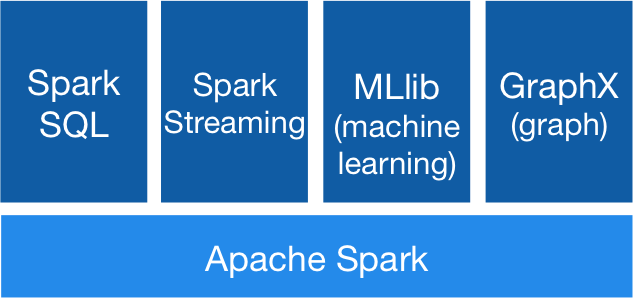
\includegraphics[width=0.7\textwidth]{spark-stack.png}
    }
    \caption{Stack applicativo Apache Spark}
    \label{fig:sparkstack}
\end{figure}




La figura \ref{fig:sparkstack} mostra le principali componenti di Apache Spark:
\begin{itemize}
\item \textbf{Spark Core}: contiene le funzionalità base di Spark fra cui l'astrazione sulla quale si basa l'intero ambiente, i \textit{resilient distributed dataset} (RDD).
\item \textbf{Spark SQL}: contiene le componenti per elaborare e manipolare dati strutturati. Permette l'interrogazione (tramite SQL) di dabatase relazionali, JSON, HIVE (mediante lo Hive Query Language) e file Parquet. 
\item \textbf{Spark Streaming}: componente che permette l'elaborazione di stream di dati.
\item \textbf{MLLib}: contiene algoritmi di Machine Learning per vari tipi di task quali classificazione, regressione, clustering, collaborative filtering, frequent pattern mining, dimensionality reduction, feature extraction e statistica di base.
\item \textbf{GraphX}: libreria per la manipolazione ed estrazione di conoscenza in grafi.
\end{itemize}

\subsection{Modello di esecuzione}
Una applicazione Spark consiste in un processo \textit{driver} e di un insieme di processi \textit{executors} distribuiti sui nodi del cluster (worker nodes) .

Il processo (nodo)   driver dovrà gestire:
\begin{itemize}
\item interazione con l'utente;
\item coordinare e distribuire il flusso di controllo.
\end{itemize}


\begin{figure}[h]
\centering
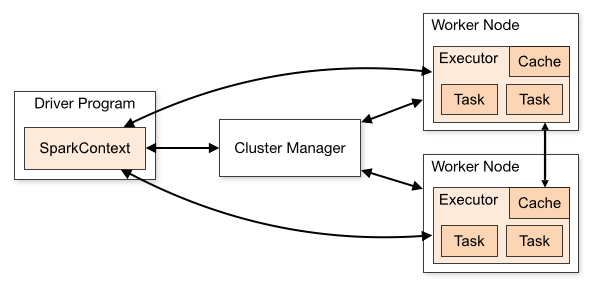
\includegraphics[width=0.8\textwidth]{cluster-ov.png}
\caption{componentiDiUnClusterSpark}
\label{fig:sparkClusterComponents}
\end{figure} 
 
I processi \lq\lq executor\rq\rq sono responsabili dell'esecuzione dei work in forma di \textit{tasks} e di memorizzare qualsiasi tipo di dato che l'utente sceglie di mantenere in cache. 

In cima al modello di esecuzione vi sono i \textit{jobs}: l'invocazione di una azione all'interno di una applicazione Spark provoca l'esecuzione di uno Spark job in grado di soddisfare la richiesta. Spark esamina il grafo degli RDD dal quale l'zione dipende e produce un piano di esecuzione che inizia computando le risorse (gli RDD) in ordine di dipendenza, culminando con l'RDD che produrrà i risultati dell'azione.
 

Il piano di esecuzione consiste nell'assemblare trasformazioni di jobs in \textit{stages}. Uno stage corrisponde a una collezione di \textit{tasks} che eseguono simultaneamente lo stesso codice su una differenze partizione dei dati: ciascuno stage contiene una sequenza di trasformazioni che possono essere completati senza rimescolare i dati.

Quest'ultimo aspetto inficia fortemente le performance dell'applicazione. Una partizione di dati subisce un processo denominato "shuffling"  quando vengono effettuate trasformazioni \textit{narrow}, ad esempio una \textit{map}.

Il trasferimento dei dati fra i nodi del cluster avviene mediante un meccanismo di serializzazione: dopo questo processo, i dati vengono memorizzati in una cache e trasferiti in rete per uno shuffling. Spark prevede due meccanismi di serializzazione: l'approccio classico (utilizzando le API Java disponibile a partire dall'interfaccia \textit{java.io.Serializable}) e mediante la libreria \textit{Kryo}. Quest'ultima prevede un formato molto più compatto in grado di svolgere le operazioni in maniera più rapida.


\section{DBpedia}
Wikipedia \footnote{https://en.wikipedia.org/} è divenuta una delle maggiori risorse di conoscenza disponibili nel web, ed è manutenuta da migliaia di utenti (collaboratori). Gli articoli Wikipedia sebbene composti prevalentemente da testo, contengono informazioni semi-strutturate come: template infobox , informazioni sulla categorizzazione dell'articolo, immagini, geo-coordinate e link sia verso altre pagine web sia verso altre pagine wikipedia.
Gli infobox sono tabelle di coppie attributo valore, che mostrano i dati più rilevanti di ciascuna pagina wikipedia. Il progetto DBpedia \cite{Bizer:2009:DCP:1640541.1640848} estrae dati strutturati da wikipedia tramite un extraction framweork open source e li unisce in una base di conoscenza multi dominio e multi lingua. Per ogni pagina presente in wikipedia, viene associato un \emph{Uniform Resource Identifier (URI)} in DBpedia per identificare un'entità o un concetto descritto dalla corrispondente pagina Wikipedia della versione inglese. Durante il processo di trasformazione, i dati semi-strutturati come i campi infobox,categorie, pagelinks sono convertiti in triple RDF e aggiunte alla base di conoscenza come proprietà dell'entità identificata dall URI.  Per rendere omogenea la descrizione delle informazioni, è stata sviluppata un ontologia e sono state definite le corrispondenze fra le proprietà presenti negli infobox e l'ontologia.
L'ontologia DBpedia consisite di 320 classi e descritte da 1650 proprietà. Le classi organizzate mediante una gerarchia sussuntiva dove \emph{owl:Thing} è la classe più generale. Poiché Il sistema di Wikipedia infobox si è evoluto in maniera decentrata, talvolta accade ad esempio che si usino diversi template per la stessa tipologia di entità (class) o si usino nomi diversi per descrive lo stesso attributo (es placeOfBirth o birthPlace). 
 L'allineamento tra i template infobox e l'ontologia a causa di queste eterogeneità presenti nella nomenclatura, non è quindi completamente automatico, ma si basa anche su mapping definiti manualmente, forniti dalla comunità di DBpedia. Ad esempio ‘date of birth’ and ‘birth
date’ sono entrambi mappati con la proprietà birthDate. 
 
 La base di conoscenza DBpedia è disponibile sul web sotto GNU Free Documentation, e può essere consultata mediante varie modalità :
\begin{itemize}
\item \textbf{Linked Data}: linked data è la metodologia di pubblicazione  dei dati RDF nel web, che utilizza gli URI http come identificativo delle risorse e il protocollo HTTP per ritrovare al descrizione rdf delle risorse. Quando si accedere ad un URI di una risorsa DBPedia mediante un semantic web agent si ottiene la descrizione rdf della risorsa mentre se si utilizza un semplice web-browser si otterrà una vista html della descrizione.
\item \textbf{Sparql Endpoint } \'E fornito un endopoint mediante il quale si può interrogare la base di conoscenza tramite il protocollo SPARQL.
\item \textbf{RDF dumps} la base di conoscenza è stata suddivisa in varie parti in base agli rdf-predicate 
\end{itemize}